\documentclass[submit]{harvardml}

% FDV: Check all frontmatter for years, due dates, and references for
% sections of the textbook, etc.
\course{CS181-S22}
\assignment{Assignment \#3}
\duedate{11:59pm EST, March 11, 2022}

\usepackage[OT1]{fontenc}
\usepackage[colorlinks,citecolor=blue,urlcolor=blue]{hyperref}
\usepackage[pdftex]{graphicx}
\usepackage{subfig}
\usepackage{fullpage}
\usepackage{amsmath}
\usepackage{amssymb}
\usepackage{color}
\usepackage{soul}
\usepackage{todonotes}
\usepackage{listings}
\usepackage{common}
\usepackage{enumitem}
\usepackage{bm}
\newcommand{\B}{\text{B}}
\newcommand{\Beta}{\text{Beta}}
\usepackage{pythonhighlight}
\usepackage[mmddyyyy,hhmmss]{datetime}


\setlength\parindent{0em}

\definecolor{verbgray}{gray}{0.9}

\lstnewenvironment{csv}{%
  \lstset{backgroundcolor=\color{verbgray},
  frame=single,
  framerule=0pt,
  basicstyle=\ttfamily,
  columns=fullflexible}}{}

\begin{document}

\begin{center}
{\Large Homework 3: Bayesian Methods and Neural Networks}\\
\end{center}

% FDV: Update for resources, accuracy of submit information **especially any colab components**
% FDV: Make sure to emphasize any plots must be in the pdf submission, we will not be checking code / source 
\subsection*{Introduction}

This homework is about Bayesian methods and Neural Networks.  Section 2.9 in the textbook as well as reviewing MLE and MAP will be useful for Q1. Chapter 4 in the textbook will be useful for Q2.

Please type your solutions after the corresponding problems using this
\LaTeX\ template, and start each problem on a new page.

Please submit the \textbf{writeup PDF to the Gradescope assignment `HW3'}. Remember to assign pages for each question.  \textbf{All plots you submit must be included in your writeup PDF.  }We will not be checking your code / source files except in special circumstances. 

Please submit your \textbf{\LaTeX file and code files to the Gradescope assignment `HW3 - Supplemental'}. 

% FDV: Last year, we pointed folks to
% https://www.cs.ubc.ca/~murphyk/Papers/bayesGauss.pdf
% and folks ended up basically copying from it and not doing any derivation
% For this year, I modified to ask folks to do the full derivation in
% 1.1 but then give them the formula for the marginal likelihood so
% they don't have to derive that.  Open to other variations:
% basically, I think it's probably okay for one part to have a longer
% derivation, but if folks think it's too much, we could have students
% refer to the paper above again or just give them the formula for 1.1
% and ask them to simply interpret it.

\newpage


\begin{problem}[Bayesian Methods]

  This question helps to build your understanding of making
  predictions with a maximum-likelihood estimation (MLE), a maximum a
  posterior estimator (MAP), and a full posterior predictive.

  Consider a one-dimensional random variable $x = \mu + \epsilon$,
  where it is known that $\epsilon \sim N(0,\sigma^2)$.  Suppose we
  have a prior $\mu \sim N(0,\tau^2)$ on the mean. You observe iid data $\{x_i\}_{i=1}^n$ (denote the data as $D$).


\textbf{We derive the distribution of $x|D$ for you.}

\textbf{The full posterior predictive is computed using:}

$$p(x|D)=\int p(x, \mu|D) d\mu =\int p(x|\mu)p(\mu|D) d\mu $$


\textbf{One can show that, in this case, the full posterior predictive distribution has a nice analytic
  form:}
   \begin{align}
        x|D \sim \mathcal{N}\Bigg(\frac{\sum_{x_i\in D}x_i}{n+\frac{\sigma^2}{\tau^2}}, (\frac{n}{\sigma^2}+\frac{1}{\tau^2})^{-1} + \sigma^2\Bigg)
     \end{align}

\begin{enumerate}

  \item Derive the distribution of $\mu|D$.

  \item 
  In many problems, it is often difficult to
  calculate the full posterior because we need to marginalize out the parameters as above (here,
  the parameter is $\mu$). We can mitigate this problem by plugging in
  a point estimate of $\mu^*$ rather than a distribution.

  a) Derive the MLE
  estimate $\mu_{MLE}$.
  % using $p(D|\mu)$.
  
  b) Derive the MAP estimate $\mu_{MAP}$. % using $p(\mu|D)$

  c) What is the relation between $\mu_{MAP}$ and the mean of $x|D$?

  d) For a fixed value of $\mu=\mu^*$, what is the distribution of $x|\mu^*$? Thus, what is the distribution of $x|\mu_{MLE}$ and $x|\mu_{MAP}$?

  e) Is the variance of $x|D$ greater or smaller than the variance of $x|\mu_{MLE}$? What is the limit of the variance of $x|D$ as $n$ tends to infinity? Explain why this is intuitive.


\item Let us compare $\mu_{MLE}$  and $\mu_{MAP}$. There are three cases to consider:

 a) Assume $\sum_{x_i \in D} x_i=0$. What are the values of $\mu_{MLE}$ and $\mu_{MAP}$?

 b) Assume $\sum_{x_i \in D} x_i>0$. Is $\mu_{MLE}$ greater than $\mu_{MAP}$?

 c) Assume $\sum_{x_i \in D} x_i<0$. Is $\mu_{MLE}$ greater than $\mu_{MAP}$?
  
    
\item Compute:

$$\lim_{n \rightarrow \infty} \frac{\mu_{MAP}}{\mu_{MLE}}$$

  \end{enumerate}

  \end{problem}

\subsection*{Solution:}
\begin{enumerate}
    \item To derive $p(\mu | D)$, we use Bayes' rule and drop terms which do not depend on $\mu$
    \begin{align}
        p(\mu | D) &\propto p(D| \mu) p(\mu) = \mathcal{N}(\mu,  \sigma^2) \mathcal{N}(0, \tau^2) \\
        &= \frac{1}{\sigma\tau \sqrt{2 \pi}} e^{\frac{-\mu^2}{2\tau^2}} \prod_{x_i \in D} e^\frac{-(x_i - \mu)^2}{2\sigma^2} \\
        & \propto e^{\frac{-\mu^2}{2\tau^2}} \prod_{x_i \in D} e^\frac{-(\mu^2 - 2x_i \mu)}{2\sigma^2} \\
        &= \prod_{x_i \in D} e^{\frac{-1}{2}{(\frac{\mu^2}{\tau^2} + \frac{\mu^2 - 2x_i \mu}{\sigma^2}})} \\
        &= \prod_{x_i \in D} e^{\frac{-1}{2\tau^2 \sigma^2}(\tau^2 \mu^2  + \sigma^2 \mu^2 - 2\tau^2 x_i\mu))}
    \end{align}
    Bringing our product into a summation within the exponential, we have
    \begin{align}
        p(\mu | D) &= e^{\frac{-1}{2\tau^2 \sigma^2}(\tau^2 \mu^2  + \sum_{i=1}^n(\sigma^2 \mu^2 - 2\tau^2 x_i\mu))} \\
        &= e^{\frac{-1}{2\tau^2 \sigma^2}((\tau^2 + n \sigma^2)\mu^2 - (2\tau^2 \sum_{i=1}^n x_i)\mu)} \\
        &= e^{\frac{-(\tau^2 + n \sigma^2)}{2\tau^2 \sigma^2}(\mu^2 - (\frac{2\tau^2 \sum_{i=1}^n x_i}{(\tau^2 + n \sigma^2)})\mu)}
    \end{align}
    By completing the square and dropping the term which does not depend on $\mu$, we get that 
    \begin{align}
        p(\mu | D) &= e^{\frac{-(\tau^2 + n \sigma^2)}{2\tau^2 \sigma^2}((\mu - \frac{\tau^2 \sum_{i=1}^n x_i}{(\tau^2 + n \sigma^2)})^2 - \frac{\tau^2 \sum_{i=1}^n x_i}{(\tau^2 + n \sigma^2)})} \\
        &\propto e^{\frac{-(\tau^2 + n \sigma^2)}{2\tau^2 \sigma^2}(\mu - \frac{\tau^2 \sum_{i=1}^n x_i}{(\tau^2 + n \sigma^2)})^2} \\
        & \implies \mu | D \sim \mathcal{N}(\frac{\tau^2 \sum_{i=1}^n x_i}{\tau^2 + n \sigma^2}, \frac{\tau^2 \sigma^2}{\tau^2 + n\sigma^2})
    \end{align}
    
    \item 
    \begin{enumerate}
        \item For our MLE estimate, we need to find $p(D | \mu*)$. Given that $x \sim \mu* + \epsilon$, it follows that 
        \begin{align}
            p(D | \mu*) &= \mathcal{N}(\mu*, \sigma^2) = \prod_{x_i \in D} \frac{1}{\sigma \sqrt{2 \pi}} e^{\frac{-(x_i - \mu*)^2}{2\sigma^2}} \\
            & \implies ln(p(D | \mu*) = \sum_{i=1}^n ln(\frac{1}{\sigma \sqrt{2 \pi}}) - \frac{(x_i - \mu*)^2}{2\sigma^2} \\
            & \implies \nabla_{\mu*} ln(p(D | \mu*) = \sum_{i=1}^n \frac{1}{2\sigma^2}(x_i - \mu*) (-2) = 0 \\
            &\implies \mu_{MLE} = \frac{1}{n}\sum_{i=1}^n x_i
        \end{align}
        \item For our MAP estimate, we need to find $p(\mu* | D) \propto p(D|\mu*) p(\mu*)$. It folows that 
        \begin{align}
            ln(p(\mu* | D)) &\propto ln(p(D| \mu*)) + ln(p(\mu*)) \\
            & = (\sum_{i=1}^n ln(\frac{1}{\sigma \sqrt{2 \pi}} - \frac{1}{2\sigma^2}(x_i - \mu*)^2) + ln(\frac{1}{\tau \sqrt{2 \pi}}) - \frac{1}{2\tau^2}\mu*^2 \\
                &\implies \nabla_{\mu*}ln(p(D|\mu*)) = (\sum_{i=1}^n \frac{-1}{2\sigma^2} (x_i - \mu*)(-2)) - \frac{1}{2\tau^2}2\mu* \\
                &= \frac{1}{\sigma^2} \sum_{i=1}^n (x_i - \mu*) - \frac{1}{\tau^2}\mu* =  \frac{1}{\sigma^2} \sum_{i=1}^n x_i - (\frac{n}{\sigma^2} + \frac{1}{\tau^2})\mu* = 0 \\
                &\implies \mu_{MAP} = \frac{1}{(n + \frac{\sigma^2}{\tau^2})} \sum_{i=1}^n x_i
        \end{align}
        \item They are the same! Our answer above matches the mean of $x|D$ exactly! 
        \item Given $ x \sim \mu* + \epsilon$, it follows that
        \begin{align}
            x | \mu* &\sim \mathcal{N}(\mu*, \sigma^2) \\
            x|\mu_{MLE} &\sim  \mathcal{N}(\frac{1}{n} \sum_{i=1}^n x_i, \sigma^2)\\
            x| \mu_{MAP} &\sim \mathcal{N}(\frac{1}{(n + \frac{\sigma^2}{\tau^2})} \sum_{i=1}^n x_i, \sigma^2)
        \end{align}
        
        \item The variance of $x | D$ is greater than the variance of $x | \mu_{MLE}$, since $(\frac{n}{\sigma^2} + \frac{1}{\tau^2})^{-1} + \sigma^2 > \sigma^2 \implies (\frac{n}{\sigma^2} + \frac{1}{\tau^2})^{-1} > 0$. \\
        As $n$ tends towards infinity, the $(\frac{n}{\sigma^2} + \frac{1}{\tau^2})^{-1}$ converges to $0$ such that the variance of $x | D$ converges to $\sigma^2$. \\
        Intuitively, we see that as we observe more input data points and $n$ grows larger, our variance of $x | D$ converges towards that of $x | \mu_{MLE}$ since more data points better sample our distribution which models our point estimate of $\mu_{MLE}$ (whereas less datapoints do not sample this distribution as closely, leading to $x |D$ having a larger variance when $n$ is not large).
        
    \end{enumerate}
    \item  We use the expressions for $\mu_{MAP}$ and $\mu_{MLE}$ derived in question 2.
    \begin{enumerate} \\
        \item $ \mu_{MLE} = \mu_{MAP} = 0 $
        \item Since $\frac{1}{n} > \frac{1}{n + \frac{\sigma^2}{\tau^2}}$, it follows that $\mu_{MAP}$ is more positive, ie $\mu_{MAP} > \mu_{MLE}$. 
        \item  Since $\frac{1}{n} > \frac{1}{n + \frac{\sigma^2}{\tau^2}}$, it follows that $-\frac{1}{n} < -\frac{1}{n + \frac{\sigma^2}{\tau^2}}$, such that $\mu_{MLE}$ is less negative, ie  $\mu_{MAP} < \mu_{MLE}$
    \end{enumerate}
    \item $\lim_{n \rightarrow \infty} \frac{\mu_{MAP}}{\mu_{MLE}} = \lim_{n \rightarrow \infty} \frac{\frac{1}{n}\sum_{x_i \in D}}{\frac{1}{n + \frac{\sigma^2}{\tau^2}}\sum_{x_i \in D}} = \lim_{n \rightarrow \infty} \frac{n + \frac{\sigma^2}{\tau^2}}{n} = 1$ 

\end{enumerate}

\newpage

\begin{problem}[Bayesian Frequentist Reconciliation]
    In this question, we connect the Bayesian version of regression with the frequentist view we have seen in the first week of class by showing how appropriate priors could correspond to regularization penalities in the frequentist world, and how the models can be different.
    
    Suppose we have a $(p+1)$-dimensional labelled dataset $\mathcal{D} = \{(\mathbf{x}_i, y_i)\}_{i=1}^N$. We can assume that $y_i$ is generated by the following random process: $$y_i = \mathbf{w}^\top\mathbf{x}_i + \epsilon_i$$ where all $\epsilon_i \sim \mathcal{N}(0,\sigma^2)$ are iid. Using matrix notation, we denote
    \begin{align*}
      \mathbf{X} &= \begin{bmatrix}\mathbf{x}_1 & \ldots & \mathbf{x}_N\end{bmatrix}^\top \in \mathbb{R}^{N \times p} \\
      \mathbf{y} &= \begin{bmatrix} y_1 & \dots & y_N \end{bmatrix}^\top  \in \mathbb{R}^N \\
      \mathbf{\epsilon} &= \begin{bmatrix} \epsilon_1 & \dots & \epsilon_N \end{bmatrix}^\top \in \mathbb{R}^N.
    \end{align*}
    
    Then we can write have $\mathbf{y} = \mathbf{X}\mathbf{w} + \mathbf{\epsilon}$. Now, we will suppose that $\mathbf{w}$ is random as well as our labels! We choose to impose the Laplacian prior $p(\mathbf{w})=\frac{1}{2\tau}\exp\left(-\frac{\|\mathbf{w}-\mathbf{\mu}\|_1}{\tau}\right)$, where $\|\mathbf{w}\|_1=\sum_{i=1}^p |w_i|$ denotes the $L^1$ norm of $\mathbf{w}$, $\mathbf{\mu}$ the location parameter, and $\tau$ is the scale factor.
    
    \begin{enumerate}
    
        \item Compute the posterior distribution $p(\mathbf{w}|\mathbf{X}, \mathbf{y})$ of $\mathbf{w}$ given the observed data $\mathbf{X}, \mathbf{y}$, up to a normalizing constant. You \textbf{do not} need to simplify the posterior to match a known distribution.
        
        \item Determine the MAP estimate $\mathbf{w}_{\mathrm{MAP}}$ of $\mathbf{w}$. You may leave the answer as the solution to an equation. How does this relate to regularization in the frequentist perspective? How does the scale factor $\tau$ relate to the corresponding regularization parameter $\lambda$? Provide intuition on the connection to regularization, using the prior imposed on $\mathbf{w}$.
        
        \item Based on the previous question, how might we incorporate prior expert knowledge we may have for the problem? For instance, suppose we knew beforehand that $\mathbf{w}$ should be close to some vector $\mathbf{v}$ in value. How might we incorporate this in the model, and explain why this makes sense in both the Bayesian and frequentist viewpoints.
        
        \item As $\tau$ decreases, what happens to the entries of the estimate $\mathbf{w}_{\mathrm{MAP}}$? What happens in the limit as $\tau \to 0$?
        
        \item Consider the point estimate $\mathbf{w}_{\mathrm{mean}}$, the mean of the posterior $\mathbf{w}|\mathbf{X},\mathbf{y}$. Further, assume that the model assumptions are correct. That is, $\mathbf{w}$ is indeed sampled from the posterior provided in subproblem 1, and that $y|\mathbf{x},\mathbf{w}\sim\mathcal{N}(\mathbf{w}^T\mathbf{x},\sigma^2)$. Suppose as well that the data generating processes for $\mathbf{x},\mathbf{w},y$ are all independent (note that $\mathbf{w}$ is random!). Between the models with estimates $\mathbf{w}_{\mathrm{MAP}}$ and $\mathbf{w}_{\mathrm{mean}}$, which model would have a lower expected test MSE, and why? Assume that the data generating distribution for $\mathbf{x}$ has mean zero, and that distinct features are independent and each have variance 1.\footnote{The unit variance assumption simplifies computation, and is also commonly used in practical applications.}
        
    \end{enumerate}
  
  
\end{problem}

\subsection*{Solution:}
\begin{enumerate}
    \item 
    \begin{align}
        p(w | X,y) &\propto p(w)p(y|X, w) = \frac{1}{2\tau}e^{-\frac{\|{w}-{\mu}\|_1}{\tau}} \frac{1}{\sqrt{(2 \pi)^{N/2}}|\Sigma|^{\frac{1}{2}}} e^{\frac{-1}{2}(y - Xw)^T \Sigma^{-1} (y-Xw)} 
    \end{align}
    where $\Sigma^{-1} = \frac{1}{\Sigma^2}I$ 
    \item 
    \begin{align}
        w_{MAP} &= argmax_w \ p(w| X,y) = argmax_w ln(p(w)) + ln(p(y|X, w)) \\
        &= argmax_w \ ln(\frac{1}{2\tau}) -\frac{\|{w}-{\mu}\|_1}{\tau} + ln(\frac{1}{\sqrt{(2 \pi)^{N/2}}|\Sigma|^{\frac{1}{2}}}) - \frac{1}{2}(y - Xw)^T \Sigma^{-1} (y-Xw) \\
         &= argmax_w \ -\frac{\|{w}-{\mu}\|_1}{\tau}  - \frac{1}{2}(y - Xw)^T \Sigma^{-1} (y-Xw) 
    \end{align}
    We see that as $\tau$ increases, we reduce emphasis on keeping $w$ close to $\mu$. This is analogous to regularization where as $\lambda$ increases, we minimize the magnitude of our weights and make them come close to $0$. In particular, the scaling by $\tau$ is very similar to Lasso regularization, except instead of driving weights to zero we are driving them to $\mu$. 
    \item Similar to regularization seen above, one way we could make $w$ close to $v$ is to use $\frac{\|{w}-{v}\|_1}{\alpha}$, where the a smaller $\alpha$ places emphasis on make $w$ be closer to $v$. Then, we would have $$w_{MAP} =  argmax_w \ \frac{\|{w}-{v}\|_1}{\alpha} +  -\frac{\|{w}-{\mu}\|_1}{\tau}  - \frac{1}{2}(y - Xw)^T \Sigma^{-1} (y-Xw) $$. \\
    Since Bayesian models begin with prior beliefs, and then update their model as they observe data, incorporating this expert knowledge makes sense since it is an instantiation of incorporating prior beliefs into our model weights. \\
    Meanwhile, although Frequentist models do not introduce priors, this expert knowledge is instead interpreted as a penalization term intended to reduce model complexity/bias.
    \item As $\tau$ decreases, the emphasis on making $w_{MAP}$ close to $\mu$ increases and the magnitude of each weight comes closer to magnitude of each component of $\mu$. As $\tau \to 0$, $w_{MAP} \to \mu$. 
\end{enumerate}

\newpage
% FDV: We had a lot of debate about this problem, whether it's useful
% for students to have to derive this by hand or not... if we want
% alternatives, ideas could include
%% (1) demonstrate the fact that there are good solutions near any
% starting point (run restarts from many starts, see that the answers
% have good quality but very different weights)
% (2) do a double-descent with linear regression (using very small N).

\begin{problem}[Neural Net Optimization]

  In this problem, we will take a closer look at how gradients are calculated for backprop with a simple multi-layer perceptron (MLP). The MLP will consist of a first fully connected layer with a sigmoid activation, followed by a one-dimensional, second fully connected layer with a sigmoid activation to get a prediction for a binary classification problem. Assume bias has not been merged. Let:
  \begin{itemize}
      \item $\bold{W}_1$ be the weights of the first layer, $\bold{b}_1$ be the bias of the first layer.
      \item $\bold{W}_2$ be the weights of the second layer, $\bold{b}_2$ be the bias of the second layer.
  \end{itemize}
  
  The described architecture can be written mathematically as: $$\hat{y} = \sigma(\bold{W}_2 \left[\sigma \left(\bold{W}_1 \bold{x} + \bold{b}_1\right)\right] + \bold{b}_2)$$
  
  where $\hat{y}$ is a scalar output of the net when passing in the single datapoint $\bold{x}$ (represented as a column vector), the additions are element-wise additions, and the sigmoid is an element-wise sigmoid.
  
  \begin{enumerate}
      \item Let:
      \begin{itemize}
          \item $N$ be the number of datapoints we have
          \item $M$ be the dimensionality of the data
          \item $H$ be the size of the hidden dimension of the first layer. Here, hidden dimension is used to describe the dimension of the resulting value after going through the layer. Based on the problem description, the hidden dimension of the second layer is 1.
      \end{itemize}
      
      Write out the dimensionality of each of the parameters, and of the intermediate variables:

          \begin{align*}
          \bold{a}_1 &= \bold{W}_1 \bold{x} + \bold{b}_1, 
          &\bold{z}_1 = \sigma(\bold{a}_1) \\
          a_2 &= \bold{W}_2 \bold{z}_1 + \bold{b}_2, 
          &\hat{y} = z_2 = \sigma(a_2)
          \end{align*}
          
      and make sure they work with the mathematical operations described above.
      
    \item  We will derive the gradients for each of the parameters.  The gradients can be used in gradient descent to find weights that improve our model's performance. For this question, assume there is only one datapoint $\bold{x}$, and that our loss is $L = -(y \log (\hat{y}) + (1 - y) \log (1 - \hat{y}))$. For all questions, the chain rule will be useful.
    \begin{enumerate}
        \item Find $\frac{\partial L}{\partial b_2}$. 
        
        \item Find $\frac{\partial L}{\partial W_2^h}$, where $W_2^h$ represents the $h$th element of $\bold{W}_2$.
        
        \item Find $\frac{\partial L}{\partial b_1^h}$, where $b_1^h$ represents the $h$th element of $\bold{b}_1$. (*Hint: Note that only the $h$th element of $\bold{a}_1$ and $\bold{z}_1$ depend on $b_1^h$ - this should help you with how to use the chain rule.)
        
        \item Find $\frac{\partial L}{\partial W_1^{h,m}}$, where  $W_1^{h,m}$ represents the element in row $h$, column $m$ in $\bold{W}_1$.
    
    \end{enumerate}
    \end{enumerate}
    
    \end{problem}

\subsection*{Solution:}
\begin{enumerate}
    \item 
    \begin{itemize}
        \item $x \in R^{Mx N} $
        \item $W_1 \in R^{HxM} $
        \item $b_1 \in R^{HxN}$
        \item $a_1 \in R^{HxN}$
        \item $z_1 \in R^{HxN}$
        \item $W_2 \in R^{1xH}$
        \item $b_2 \in R^{1xN}$
        \item $a_2 \in R^{1xN}$
        \item $z_2 \in R^{1xN}$
    \end{itemize}
    
    \item
    \begin{enumerate}
        \item 
        \begin{align}
            \frac{\partial L}{\partial b_2} &= \frac{\partial L}{\partial \hat y}\frac{\partial \hat y}{\partial a_2} \frac{\partial a_2}{\partial b_2} = [-(\frac{y}{\hat y} + \frac{y-1}{1-\hat y})] \ [\hat y (1 - \hat y)] \ [1] = y(\hat y - 1) + \hat y (1 - y)
        \end{align}
        \item 
        \begin{align}
            \frac{\partial L}{\partial W_2^h} &= [\frac{\partial L}{\partial \hat y}\frac{\partial \hat y}{\partial a_2}] \frac{\partial a_2}{\partial W_2^h} = [y(\hat y - 1) + \hat y (1 - y)] \ z_1^h
        \end{align}
        \item
        \begin{align}
            \frac{\partial L}{\partial b_1^h} &= [\frac{\partial L}{\partial \hat y}\frac{\partial \hat y}{\partial a_2} ] \frac{\partial a_2}{\partial z_1^h} \frac{\partial z_1^h}{\partial a_1^h} \frac{\partial a_1^h }{\partial b_1^h} = [y(\hat y - 1) + \hat y (1 - y)] \ [w_2^h] \ [z_1^h (1 - z_1^h)] \ [1] \\
            &= [y(\hat y - 1) + \hat y (1 - y)] \ [w_2^h] \ [z_1^h (1 - z_1^h)]
        \end{align}
        \item 
        \begin{align}
            \frac{\partial L}{\partial W_1^{h,m}} &= [\frac{\partial L}{\partial \hat y}\frac{\partial \hat y}{\partial a_2}  \frac{\partial a_2}{\partial z_1^h} \frac{\partial z_1^h}{\partial a_1^h}] \frac{\partial a_1^h }{\partial W_1^{h,m}} = [y(\hat y - 1) + \hat y (1 - y)] \ [w_2^h] \ [z_1^h (1 - z_1^h)] \ [x^m]
        \end{align}
    \end{enumerate}
\end{enumerate}



\newpage

\begin{problem}[Modern Deep Learning Tools: PyTorch]
  In this problem, you will learn how to use PyTorch. This machine learning library is massively popular and used heavily throughout industry and research. In \verb|T3_P3.ipynb| you will implement an MLP for image classification from scratch. Copy and paste code solutions below and include a final graph of your training progress. Also submit your completed \verb|T3_P3.ipynb| file.

  {\bfseries You will recieve no points for code not included below.}

  {\bfseries You will recieve no points for code using built-in APIs from the \verb|torch.nn| library.}
  
\end{problem}


\subsection*{Solution:}
Plot:

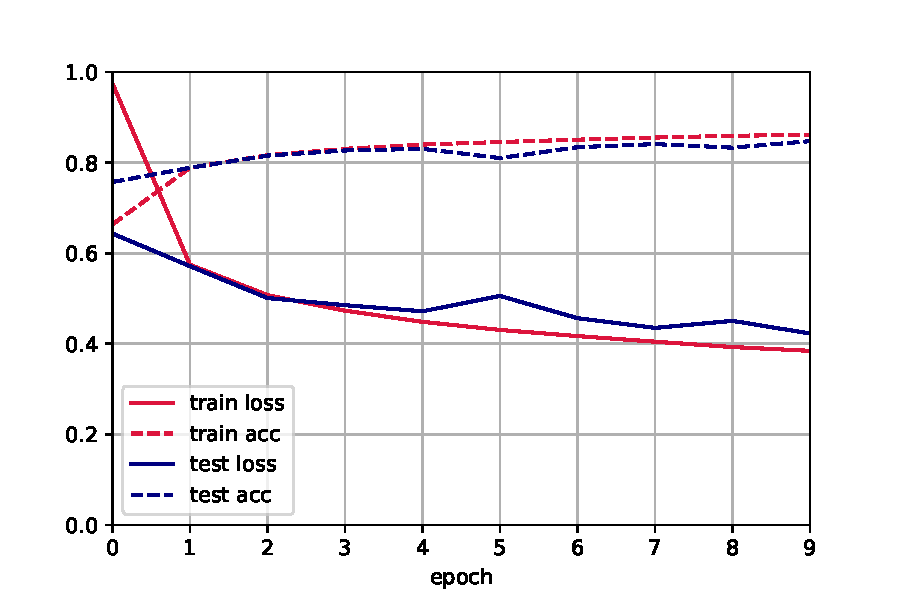
\includegraphics[width=\linewidth]{final_plot}

Code:

\begin{python}
# given a single image (M=1)
n_inputs = 28*28  # D
n_hiddens = 256  # J
n_outputs = 10     # number of possible labels

W1 = torch.nn.Parameter(torch.randn(size=(n_inputs, n_hiddens)))
b1 = torch.nn.Parameter(torch.randn(size=(1, n_hiddens)))
W2 = torch.nn.Parameter(torch.randn(size=(n_hiddens, n_outputs)))
b2 = torch.nn.Parameter(torch.randn(size=(1, n_outputs)))

# needed to prevent initial weights being too large.. nan errors
with torch.no_grad():
    W1 *= 0.01
    W2 *= 0.01
    
params = [W1, b1, W2, b2]



def relu(x):
    return torch.clamp(x, min=0)

def softmax(X):
    # unsqueeze puts denominator on axis and divides, preserves tensor allowing for summation and division
    return torch.div(torch.exp(X), torch.sum(torch.exp(X), dim=1).unsqueeze(1))


# forward pass net(X) expects X to be a batch of FashionMNIST, hence the shape (batch_size, 1, 28, 28).
def net(X):
    # flatten first image of batch
    x = torch.flatten(X[0]).reshape(1,-1)
    # for remaining images in the batch, flatten and stack together
    for i in range(1, X.shape[0]):
        x = torch.cat([x, torch.flatten(X[i]).reshape(1,-1)], axis=0)
        
    H = relu(x @ W1 + b1)
    O = softmax(H @ W2 + b2)
    
    return O


def cross_entropy(y_hat, y):
    mesh = torch.gather(y_hat, 1, y.unsqueeze(1))   # gather values along first dimension so that we can take the log
    return -1 * torch.log(mesh)

def sgd(params, lr=0.1):
    with torch.no_grad():
        for i in range(0, len(params)):
            # note that x = x-1 is not the same as x -= 1... later modifies same tensor, 
            # while first makes new tensor and throws error!
            params[i] -= lr * params[i].grad
        # have to zero out gradients once all backpropogation is complete, not before
        for i in range(0, len(params)):
            params[i].grad.zero_()


# modelled based off of training code
def train(net, params, train_iter, loss_func=cross_entropy, updater=sgd):
    for _ in tqdm(range(epochs)):
        for X, y in train_iter:
            y_hat = net(X)
            loss = loss_func(y_hat, y).mean()
            loss.backward()
            updater(params)
\end{python}


\newpage
%%%%%%%%%%%%%%%%%%%%%%%%%%%%%%%%%%%%%%%%%%%%%
% Name and Calibration
%%%%%%%%%%%%%%%%%%%%%%%%%%%%%%%%%%%%%%%%%%%%%
\subsection*{Name}
Arnav Srivastava

\subsection*{Collaborators and Resources}
Collaborated with Chinmay Deshpande and Jeremy Zhang. \\
Resource: https://stackoverflow.com/questions/57237352/what-does-unsqueeze-do-in-pytorch

\subsection*{Calibration}
Approximately how long did this homework take you to complete (in hours)? \\
20

\end{document}
